%%%%%%%%%%%%%%%%%%%%%%%%%%%%%%%%%%%%%%%%%%%%%%%%%%%%%%%%%%%%%%%%%%%%%%
%% Classical ML for Binary Diabetes Risk Prediction
%% Course format (格式要求): Arial/Helvetica 11 pt, double spacing,
%% margins 2.5/2.5/2.5/2.0 cm, continuous page numbers.
%% Architecture mirrors Springer Nature template.tex front matter
%% (title / author / affil / abstract / keywords / numbered sections /
%% appendix / APA references) without requiring sn-jnl.cls.
%%%%%%%%%%%%%%%%%%%%%%%%%%%%%%%%%%%%%%%%%%%%%%%%%%%%%%%%%%%%%%%%%%%%%%
\documentclass[11pt,a4paper]{article}

%%%% Core packages
\usepackage[T1]{fontenc}
\usepackage[utf8]{inputenc}
\usepackage{amsmath,amssymb}
\usepackage{graphicx}
\usepackage{booktabs}
\usepackage{multirow}
\usepackage{xcolor}
\usepackage{textcomp}
\usepackage{listings}
\usepackage[title]{appendix}
\usepackage{url}
\usepackage[authoryear,round]{natbib}
\usepackage[hidelinks]{hyperref}
\usepackage{enumitem}

%%%% Course formatting overlay (格式要求.txt)
\usepackage{helvet}% Arial-compatible under pdfLaTeX
\renewcommand{\familydefault}{\sfdefault}
\usepackage{courier}% monospace for code
\usepackage[top=2.5cm,bottom=2.0cm,left=2.5cm,right=2.5cm]{geometry}
\usepackage{setspace}
\doublespacing
\usepackage{ragged2e}
\justifying
\usepackage{fancyhdr}
\pagestyle{fancy}
\fancyhf{}
\fancyfoot[C]{\thepage}
\renewcommand{\headrulewidth}{0pt}
\renewcommand{\footrulewidth}{0pt}
\renewcommand{\normalsize}{\fontsize{11}{22}\selectfont}
\normalsize

%%%% Code listings (course: monospace + light gray)
\definecolor{codebg}{RGB}{245,245,245}
\lstset{%
  basicstyle=\small\ttfamily,%
  backgroundcolor=\color{codebg},%
  frame=single,%
  framesep=4pt,%
  breaklines=true,%
  columns=fullflexible%
}

%%%% Template-like front-matter helpers (article stand-in for sn-jnl)
\newcommand{\fnm}[1]{#1}
\newcommand{\sur}[1]{#1}
\providecommand{\keywords}[1]{%
  \par\vspace{0.5\baselineskip}%
  \noindent\textbf{Keywords:} #1\par
}
%% Author / affiliation block (must use \makeatletter because of \@...)
\makeatletter
\newcommand{\courseauthor}[1]{\def\@courseauthor{#1}}
\newcommand{\courseaffil}[1]{\def\@courseaffil{#1}}
\newcommand{\coursesubtitle}[1]{\def\@coursesubtitle{#1}}
\newcommand{\coursegithub}[1]{\def\@coursegithub{#1}}
\newcommand{\makecoursetitle}{%
  \thispagestyle{empty}%
  \begin{center}
    {\Large\bfseries \@title\par}
    \vspace{1.0\baselineskip}
    {\large \@coursesubtitle\par}
    \vspace{1.5\baselineskip}
    {\normalsize Course: \@courseaffil\par}
    \vspace{0.75\baselineskip}
    {\normalsize Author: \@courseauthor\par}
    \vspace{0.75\baselineskip}
    {\normalsize GitHub: \expandafter\url\expandafter{\@coursegithub}\par}
  \end{center}
  \vspace{1.0\baselineskip}
}
\makeatother

\graphicspath{{files/pic/}}

\begin{document}

%%%%%%%%%%%%%%%%%%%%%%%%%%%%%%%%%%%%%%%%%%%%%%%%%%%%%%%%%%%%%%%%%%%%%%
%% Title block (template.tex architecture)
%%%%%%%%%%%%%%%%%%%%%%%%%%%%%%%%%%%%%%%%%%%%%%%%%%%%%%%%%%%%%%%%%%%%%%
\title{Classical ML for Binary Diabetes Risk Prediction}
\coursesubtitle{A benchmarking study on the CDC BRFSS 2015 Diabetes Health Indicators dataset}
\courseaffil{MDS 5 -- Predictive Analytics}
\courseauthor{Yue Ma}
\coursegithub{https://github.com/nikk909/mds5_Income_prediction}

\makecoursetitle

\begin{abstract}
\noindent
This study benchmarks five classical machine learning algorithms---logistic regression, k-nearest neighbors (KNN), decision tree, random forest, and linear support vector machine---for binary diabetes risk prediction on a stratified 50,000-record subset of the BRFSS 2015 Diabetes Health Indicators dataset. After removing duplicates, about 48,003 rows remain, with roughly 83.6\% negative and 16.4\% positive cases. The pipeline includes quality checks, a stratified 80/20 split, Pearson Top-8 feature selection on the training set only, and StandardScaler fitted on training data. Models are compared by Accuracy, Precision, Recall, F1-score, and AUC. Without class weighting, Accuracy is high (about 0.82--0.84) but positive-class Recall is low; KNN has the highest F1 (0.2964), while linear models lead in AUC (about 0.807). Enabling \lstinline{class_weight='balanced'} for logistic regression and random forest raises Recall to about 0.70--0.75 and F1 to about 0.47, while Accuracy falls. For screening-oriented tasks, model choice should prioritize F1, AUC, and Recall together with imbalance handling, not Accuracy alone. A balanced logistic regression is a practical recommendation when minority detection matters.
\end{abstract}

\keywords{binary classification, diabetes risk, BRFSS, class imbalance, classical machine learning, F1-score, ROC-AUC}

\clearpage
\pagestyle{fancy}

%%%%%%%%%%%%%%%%%%%%%%%%%%%%%%%%%%%%%%%%%%%%%%%%%%%%%%%%%%%%%%%%%%%%%%
\section{Introduction}\label{sec:intro}
%%%%%%%%%%%%%%%%%%%%%%%%%%%%%%%%%%%%%%%%%%%%%%%%%%%%%%%%%%%%%%%%%%%%%%

Diabetes is a chronic condition. Early identification of high-risk groups supports lifestyle intervention and efficient use of preventive care. When survey-based data are used for prediction, two difficulties appear: labels reflect self-reported status rather than clinical confirmation, and class imbalance is strong---most respondents are non-diabetic, yet the minority class is clinically important. Optimizing Accuracy alone tends to favor the majority class: the model looks accurate while missing many at-risk individuals.

This study uses the Kaggle Diabetes Health Indicators dataset derived from the CDC BRFSS 2015 \citep{CDC2015,TeboulND}. Original multi-class labels are merged into a binary target \texttt{Diabetes\_binary} (0 = no diabetes; 1 = prediabetes or diagnosed). A stratified sample of 50,000 records is drawn (\lstinline{random_state=42}), preserving roughly an 84\%/16\% class ratio. The predictive question is: given blood pressure, cholesterol, BMI, age, general health, and related indicators, can we estimate binary diabetes risk?

Five classical algorithms are compared under a fixed protocol, with emphasis on metric choice under imbalance. The central research question is: on BRFSS-style binary diabetes risk data, which classical models perform better when F1, AUC, and Recall are considered jointly---rather than Accuracy alone---and can class weighting improve minority detection?

The remainder of the paper is organized as follows. Section~\ref{sec:theory} reviews theory and academic debate; Section~\ref{sec:method} describes data, preprocessing, and the experimental protocol; Section~\ref{sec:analysis} presents analysis anchored in project figures and tables; Section~\ref{sec:conclusion} concludes. Code and figures are available in the GitHub repository (\lstinline{diabetes_ml_benchmark.ipynb}; \texttt{files/pic} and \texttt{files/data}).

%%%%%%%%%%%%%%%%%%%%%%%%%%%%%%%%%%%%%%%%%%%%%%%%%%%%%%%%%%%%%%%%%%%%%%
\section{Theory: State of Research and Academic Debate}\label{sec:theory}
%%%%%%%%%%%%%%%%%%%%%%%%%%%%%%%%%%%%%%%%%%%%%%%%%%%%%%%%%%%%%%%%%%%%%%

\subsection{Diabetes risk prediction and health survey data}\label{sec:theory-data}

Population screening for diabetes risk often relies on hypertension, dyslipidemia, BMI, physical activity, and self-rated general health \citep{ADA2021}. These indicators are not laboratory gold standards but are suitable for large survey-based risk stratification.

The Behavioral Risk Factor Surveillance System (BRFSS) is widely used in applied machine learning for health outcomes. Strengths include standardized questionnaires and large samples; limitations include self-report bias and cross-sectional design. Model outputs should be interpreted as population risk signals for screening, not clinical diagnosis.

A recurring debate contrasts interpretable linear models (e.g., logistic regression) with more flexible tree ensembles (e.g., random forests). Linear models offer transparency; ensembles often improve ranking metrics such as AUC. Univariate Pearson correlation and forest importances need not agree---they capture different aspects of association.

BRFSS diabetes features are largely numeric or low-cardinality ordinal variables. Label encoding is therefore unnecessary; standardization and imbalance handling are the main methodological focus.

\subsection{Supervised learning formulations}\label{sec:theory-sl}

Supervised learning maps labeled inputs to predictions for unseen cases \citep{James2021}. This benchmark compares five classical algorithms under one protocol.

\subsubsection{Logistic regression}

Binary logistic regression models
\begin{equation}
P(y=1\mid x)=\frac{1}{1+\exp(-(w^{\top}x+b))}.
\end{equation}
Parameters are estimated via maximum likelihood (cross-entropy loss) \citep{Hosmer2013}. Coefficients support interpretation when features are on comparable scales. \lstinline{class_weight='balanced'} adjusts for skewed priors. In screening settings, weighted logistic regression is often a strong, interpretable baseline for AUC and recall trade-offs.

\subsubsection{K-nearest neighbors (KNN)}

KNN classifies a point by majority vote among its $k$ nearest neighbors in feature space. Predictions depend on local geometry; features should be scaled. With about 16\% positives, KNN ($k=5$) can achieve relatively high local F1 at default thresholds but may trail linear models in AUC, reflecting weaker global ranking of risk.

\subsubsection{Decision tree}

Decision trees partition the feature space recursively using impurity criteria such as Gini. They capture non-linear interactions but overfit easily. \lstinline{max_depth=10} is a common regularizer. In this project, a single tree sits between KNN and ensemble performance.

\subsubsection{Random forest}

Random forests \citep{Breiman2001} aggregate bagged trees with random feature subsets, reducing variance via voting. They handle non-linearity and provide feature importances. Under severe imbalance without weighting, forests may favor the majority class for Accuracy; \lstinline{class_weight='balanced'} should be evaluated explicitly.

\subsubsection{Linear support vector machine}

Support vector machines seek a maximum-margin separator \citep{Cortes1995}. This study uses \lstinline{LinearSVC} with \lstinline{decision_function} scores for AUC. Linear SVM and logistic regression often perform similarly on ranking metrics; choosing a linear kernel avoids heavy RBF training cost while preserving interpretability of linear boundaries in scaled space.

\subsection{Feature selection: Pearson correlation filter}\label{sec:theory-pearson}

Pearson correlation ranks linear association with the binary target. Top-$k$ filtering is simple and reproducible but captures only linear relationships and can miss redundant predictors. Features are selected on the training set only after stratified splitting to avoid leakage---consistent with the Pearson Top-8 protocol in Section~\ref{sec:method}.

\subsection{Class imbalance: metrics and remedies}\label{sec:theory-imbalance}

When negatives dominate, Accuracy is misleading; Precision, Recall, and F1 better reflect minority performance \citep{He2009}. ROC-AUC summarizes ranking but does not alone specify operating points \citep{Fawcett2006}. Remedies include algorithm-level class weights, resampling (e.g., SMOTE; \citealp{Chawla2002}), and threshold tuning. This project emphasizes \lstinline{class_weight} ablation for logistic regression and random forest.

\subsection{Evaluation protocol and validity}\label{sec:theory-eval}

Fair comparison requires fixed splits, preprocessing fit on training data only, and consistent metrics. Internal validity holds when all models share \lstinline{random_state=42}, stratified \lstinline{test_size=0.2}, and the same Top-8 features. External validity to other populations remains limited by BRFSS sampling and self-report.

\subsection{Synthesis for this application}\label{sec:theory-synth}

For BRFSS binary diabetes screening: (1)~enforce leakage-safe preprocessing; (2)~prioritize F1, AUC, and Recall over Accuracy; (3)~report both linear and ensemble models and compare correlation filters with forest importances. Section~\ref{sec:analysis} applies these principles to empirical results.

%%%%%%%%%%%%%%%%%%%%%%%%%%%%%%%%%%%%%%%%%%%%%%%%%%%%%%%%%%%%%%%%%%%%%%
\section{Methodology}\label{sec:method}
%%%%%%%%%%%%%%%%%%%%%%%%%%%%%%%%%%%%%%%%%%%%%%%%%%%%%%%%%%%%%%%%%%%%%%

\subsection{Research design and aim}\label{sec:method-design}

This is a supervised learning benchmarking study: under a fixed protocol, five classical classifiers are compared to answer which models are better for which metrics and why. No causal claims or clinical trial inference are made.

\subsection{Data source and sample}\label{sec:method-data}

The Kaggle Diabetes Health Indicators Dataset reflects BRFSS 2015 \citep{TeboulND}; about 253,680 rows. Script \lstinline{dataset/make_binary_50k.py} maps \texttt{Diabetes\_012} to \texttt{Diabetes\_binary} (0 vs.\ merged 1/2), draws a stratified 50,000-row sample (\lstinline{random_state=42}), and deduplicates before modeling (48,003 rows: 40,138 negatives, 7,865 positives; Figure~\ref{fig:classbalance}).

Features are numeric or ordinal (Age, Education, Income, GenHlth, BMI, MentHlth, PhysHlth, etc.). As in the Adult income workflow, categorical ordinals are treated numerically without label encoding; emphasis is on scaling and imbalance handling.

\subsection{Data quality and cleaning}\label{sec:method-qc}

Checks include missing values, duplicate rows, and plausible ranges (BMI in $[10,60]$; MentHlth/PhysHlth in $[0,30]$). Duplicate rows are removed to avoid inflating performance.

\subsection{Splitting, feature selection, and scaling}\label{sec:method-split}

\lstinline{train_test_split(test_size=0.2, stratify=y, random_state=42)} creates hold-out test data. Pearson correlation with the target on the training set selects Top-8 features (Table~\ref{tab:top8}). \lstinline{StandardScaler} is fit on training features and applied to train and test for distance- and margin-based models.

\begin{table}[htbp]
\centering
\caption{Pearson Top-8 features (training set).}
\label{tab:top8}
\begin{tabular}{lrr}
\toprule
Feature & Pearson $r$ & $|r|$ \\
\midrule
GenHlth & 0.2900 & 0.2900 \\
HighBP & 0.2648 & 0.2648 \\
BMI & 0.2208 & 0.2208 \\
DiffWalk & 0.2090 & 0.2090 \\
HighChol & 0.2059 & 0.2059 \\
Age & 0.1832 & 0.1832 \\
HeartDiseaseorAttack & 0.1702 & 0.1702 \\
Income & $-0.1634$ & 0.1634 \\
\bottomrule
\end{tabular}
\end{table}

\subsection{Models and hyperparameters}\label{sec:method-models}

Logistic regression (\lstinline{max_iter=1000}), KNN (\lstinline{n_neighbors=5}), decision tree (\lstinline{max_depth=10}), random forest (\lstinline{n_estimators=100}, \lstinline{max_depth=12}), and \lstinline{LinearSVC} (\lstinline{max_iter=2000}) share the same feature matrix. Imbalance ablation compares default weights with \lstinline{class_weight='balanced'} for logistic regression and random forest.

\subsection{Metrics, artifacts, and reproducibility}\label{sec:method-metrics}

Test-set Accuracy, Precision, Recall, F1, AUC, and training time are recorded. Figures are saved under \texttt{files/pic/}; metric tables under \texttt{files/data/}. The full pipeline is implemented in \lstinline{diabetes_ml_benchmark.ipynb} on GitHub.

%%%%%%%%%%%%%%%%%%%%%%%%%%%%%%%%%%%%%%%%%%%%%%%%%%%%%%%%%%%%%%%%%%%%%%
\section{Analysis \& Discussion}\label{sec:analysis}
%%%%%%%%%%%%%%%%%%%%%%%%%%%%%%%%%%%%%%%%%%%%%%%%%%%%%%%%%%%%%%%%%%%%%%

\subsection{Class distribution}\label{sec:analysis-balance}

After deduplication, negatives are 40,138 (83.6\%) and positives 7,865 (16.4\%)---roughly a five-to-one ratio. A majority-class baseline already yields Accuracy near 0.84, so Accuracy alone must not drive model selection.

\begin{figure}[htbp]
\centering
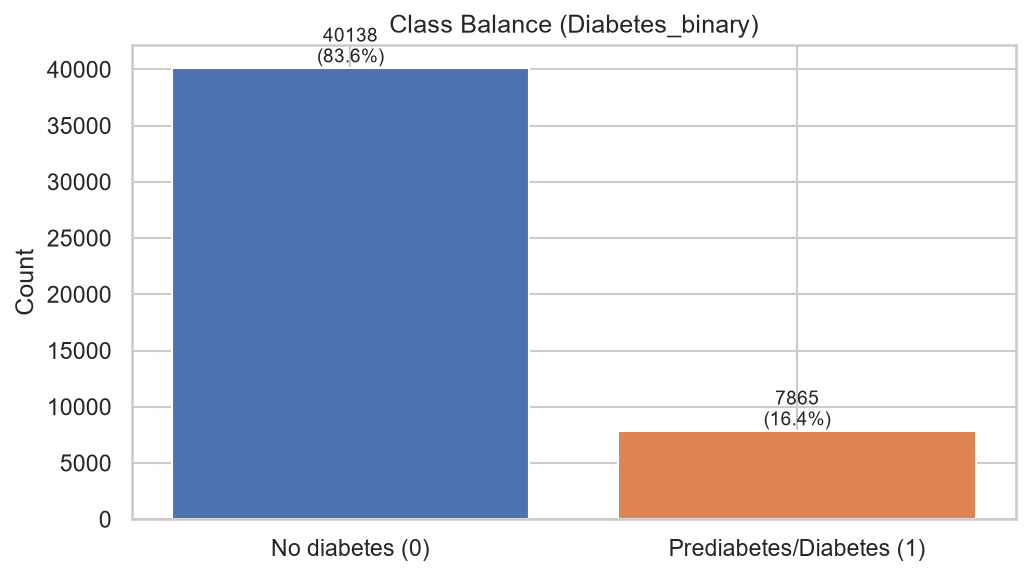
\includegraphics[width=0.85\textwidth]{class_balance.png}
\caption{Class balance of \texttt{Diabetes\_binary}.}
\label{fig:classbalance}
\end{figure}

\subsection{Distributions, correlation, and Table~\ref{tab:top8}}\label{sec:analysis-eda}

Figure~\ref{fig:hist} shows skewed BMI and health burden variables, motivating \lstinline{StandardScaler} for LR, KNN, and SVM. Figure~\ref{fig:box} separates classes for BMI, GenHlth, Age, and Income---higher BMI and worse GenHlth align with positive labels. Figure~\ref{fig:corr} and Table~\ref{tab:top8} agree that GenHlth, HighBP, BMI, DiffWalk, and HighChol rank highest; Income is negatively correlated, consistent with socioeconomic gradients in survey data.

\begin{figure}[htbp]
\centering
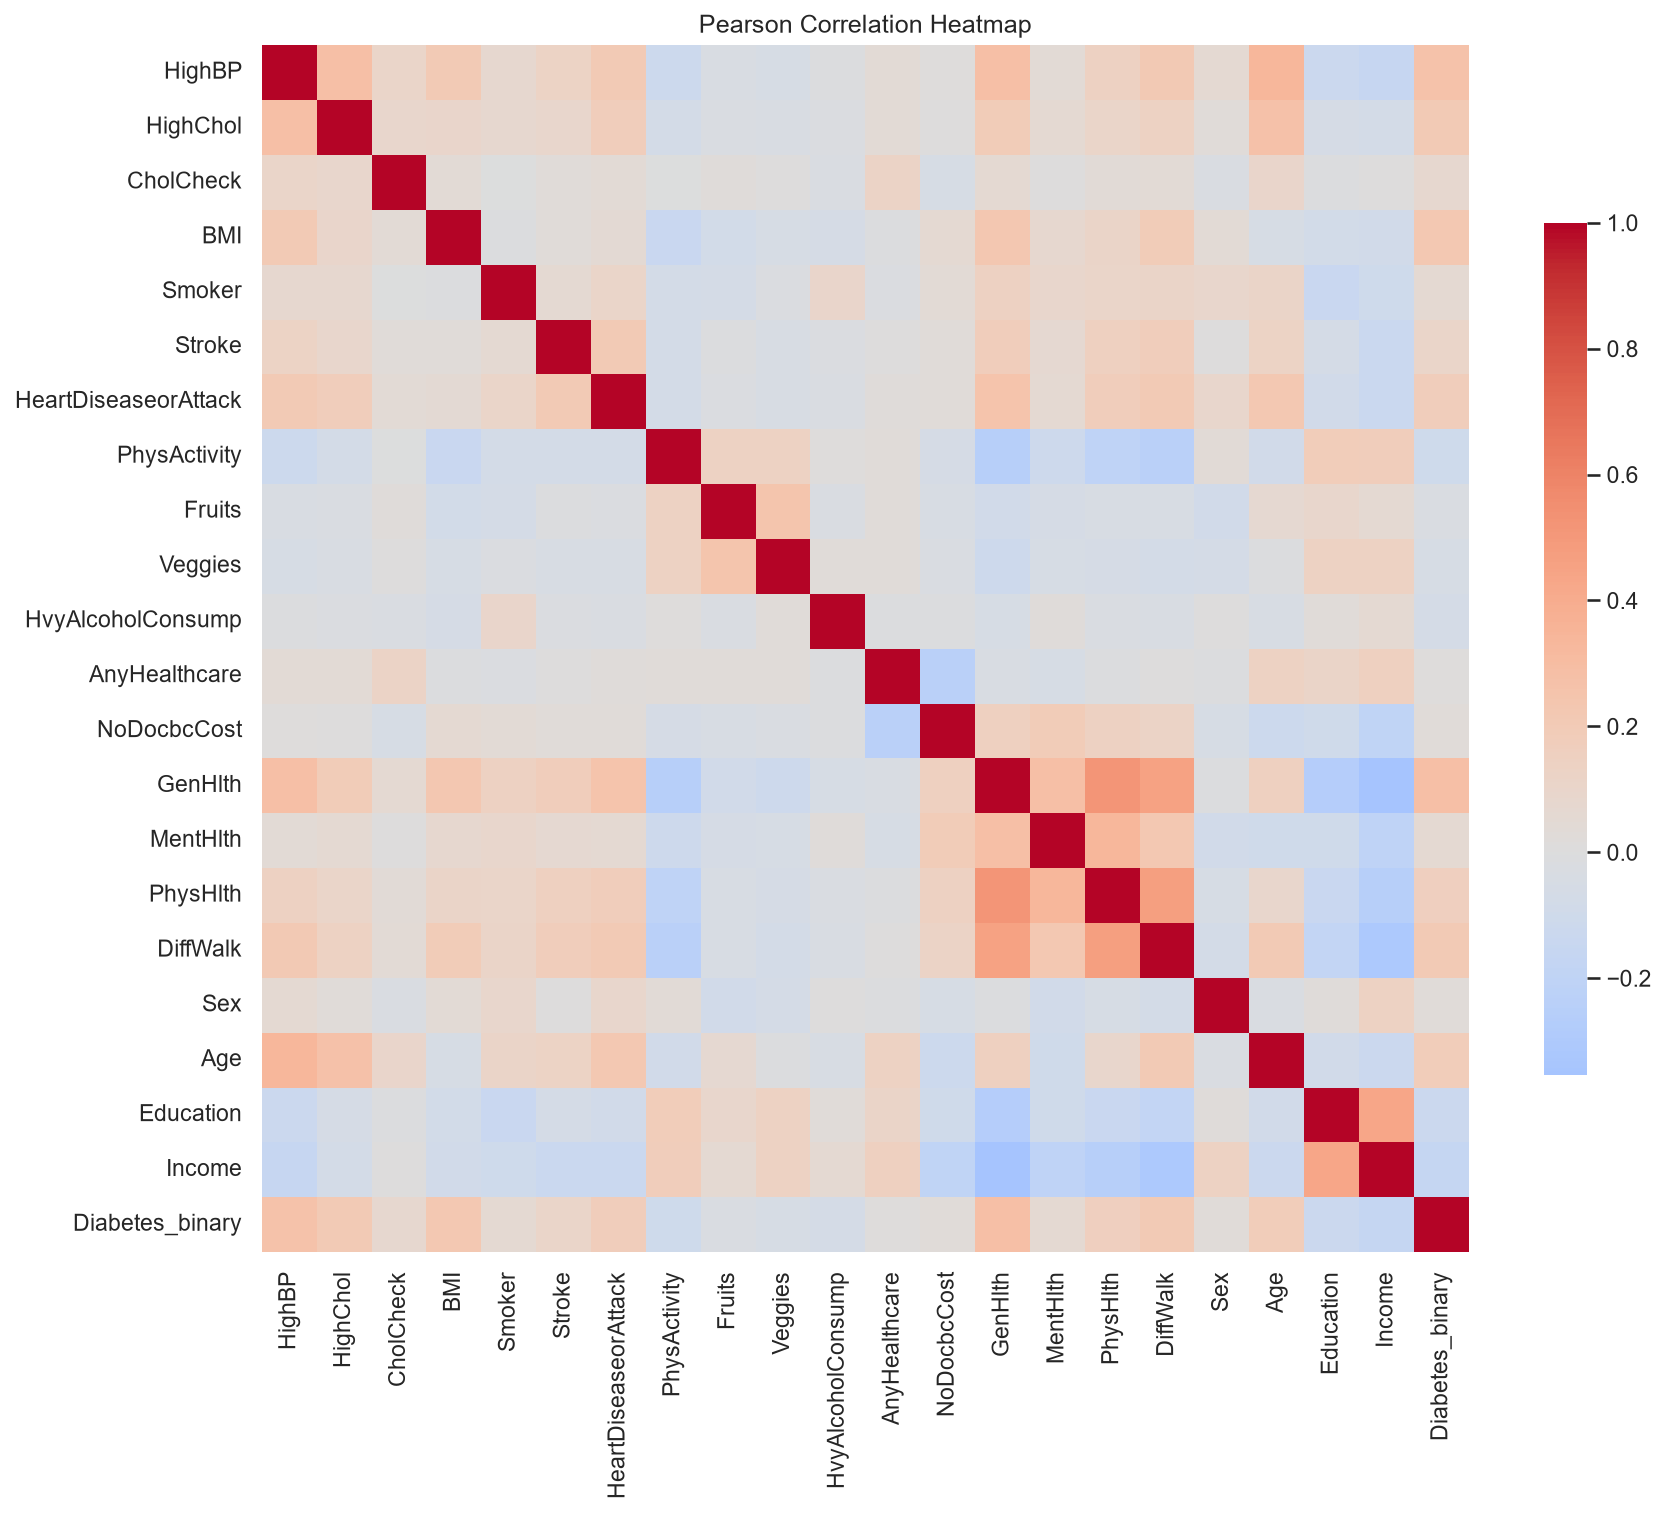
\includegraphics[width=0.85\textwidth]{correlation_heatmap.png}
\caption{Pearson correlation heatmap.}
\label{fig:corr}
\end{figure}

\begin{figure}[htbp]
\centering
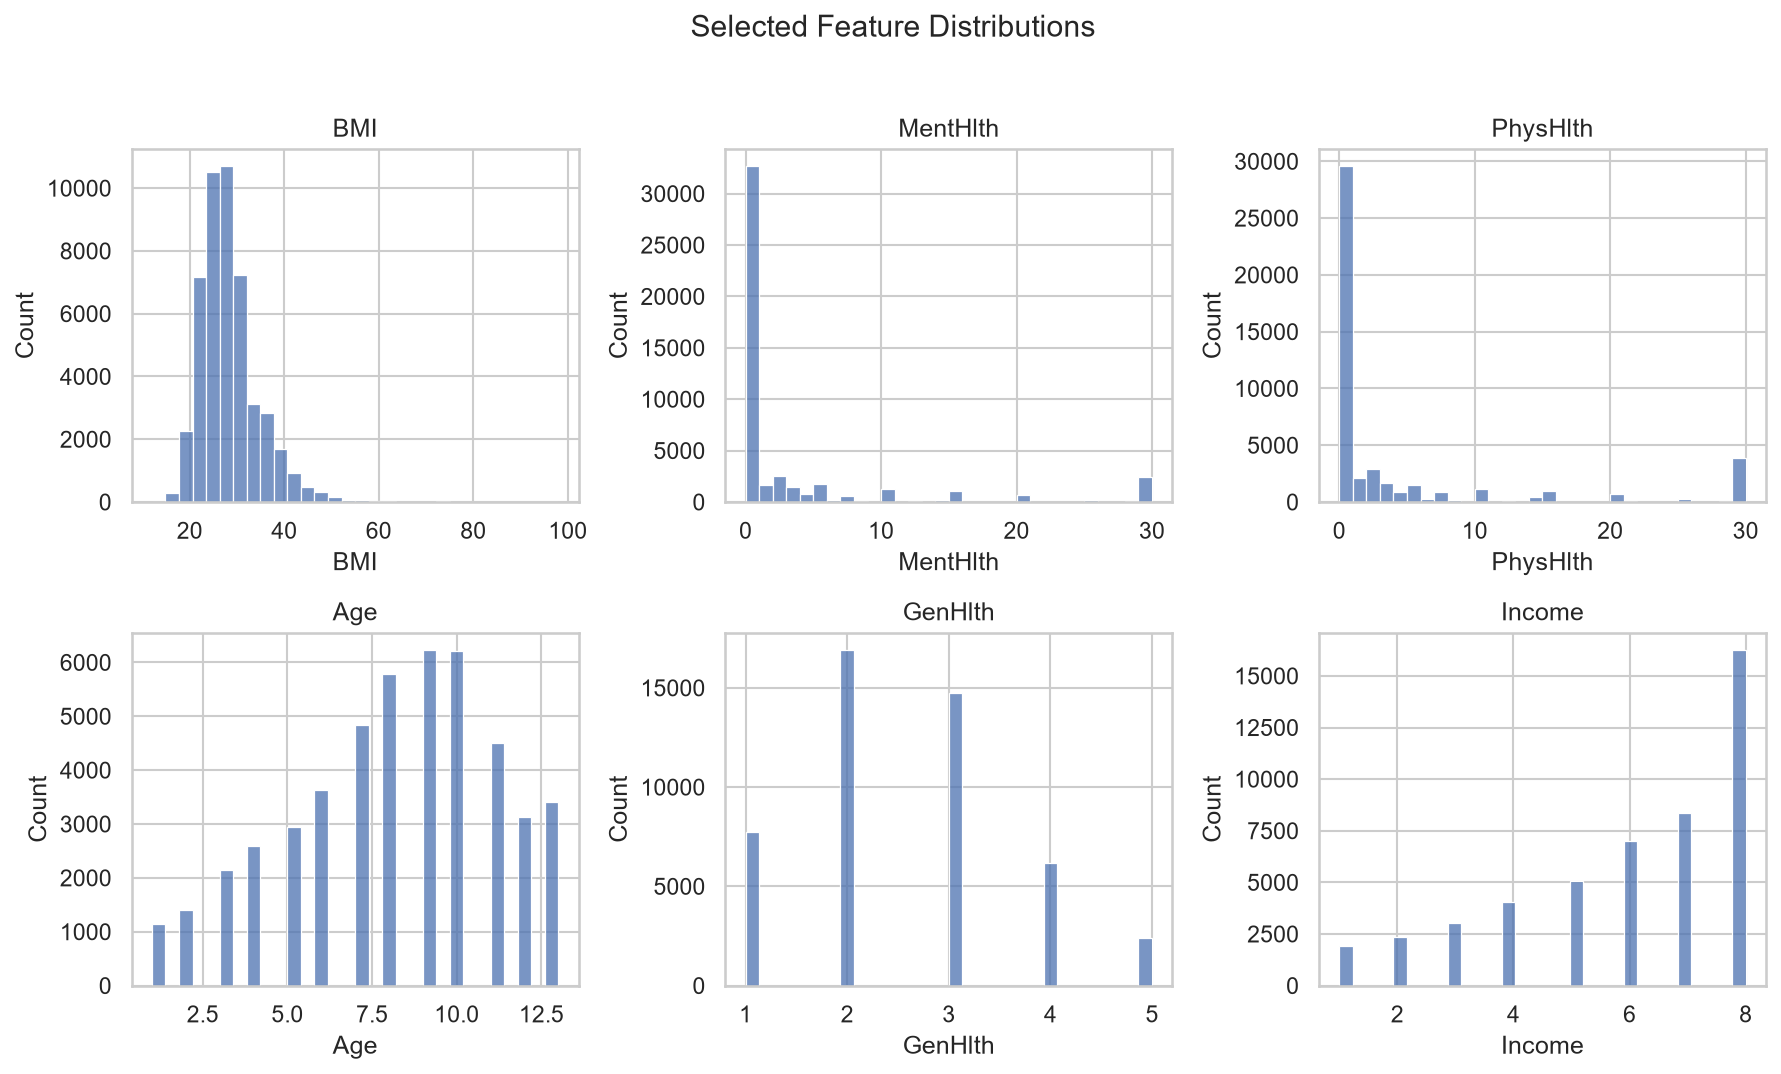
\includegraphics[width=0.85\textwidth]{feature_histograms.png}
\caption{Selected feature histograms.}
\label{fig:hist}
\end{figure}

\begin{figure}[htbp]
\centering
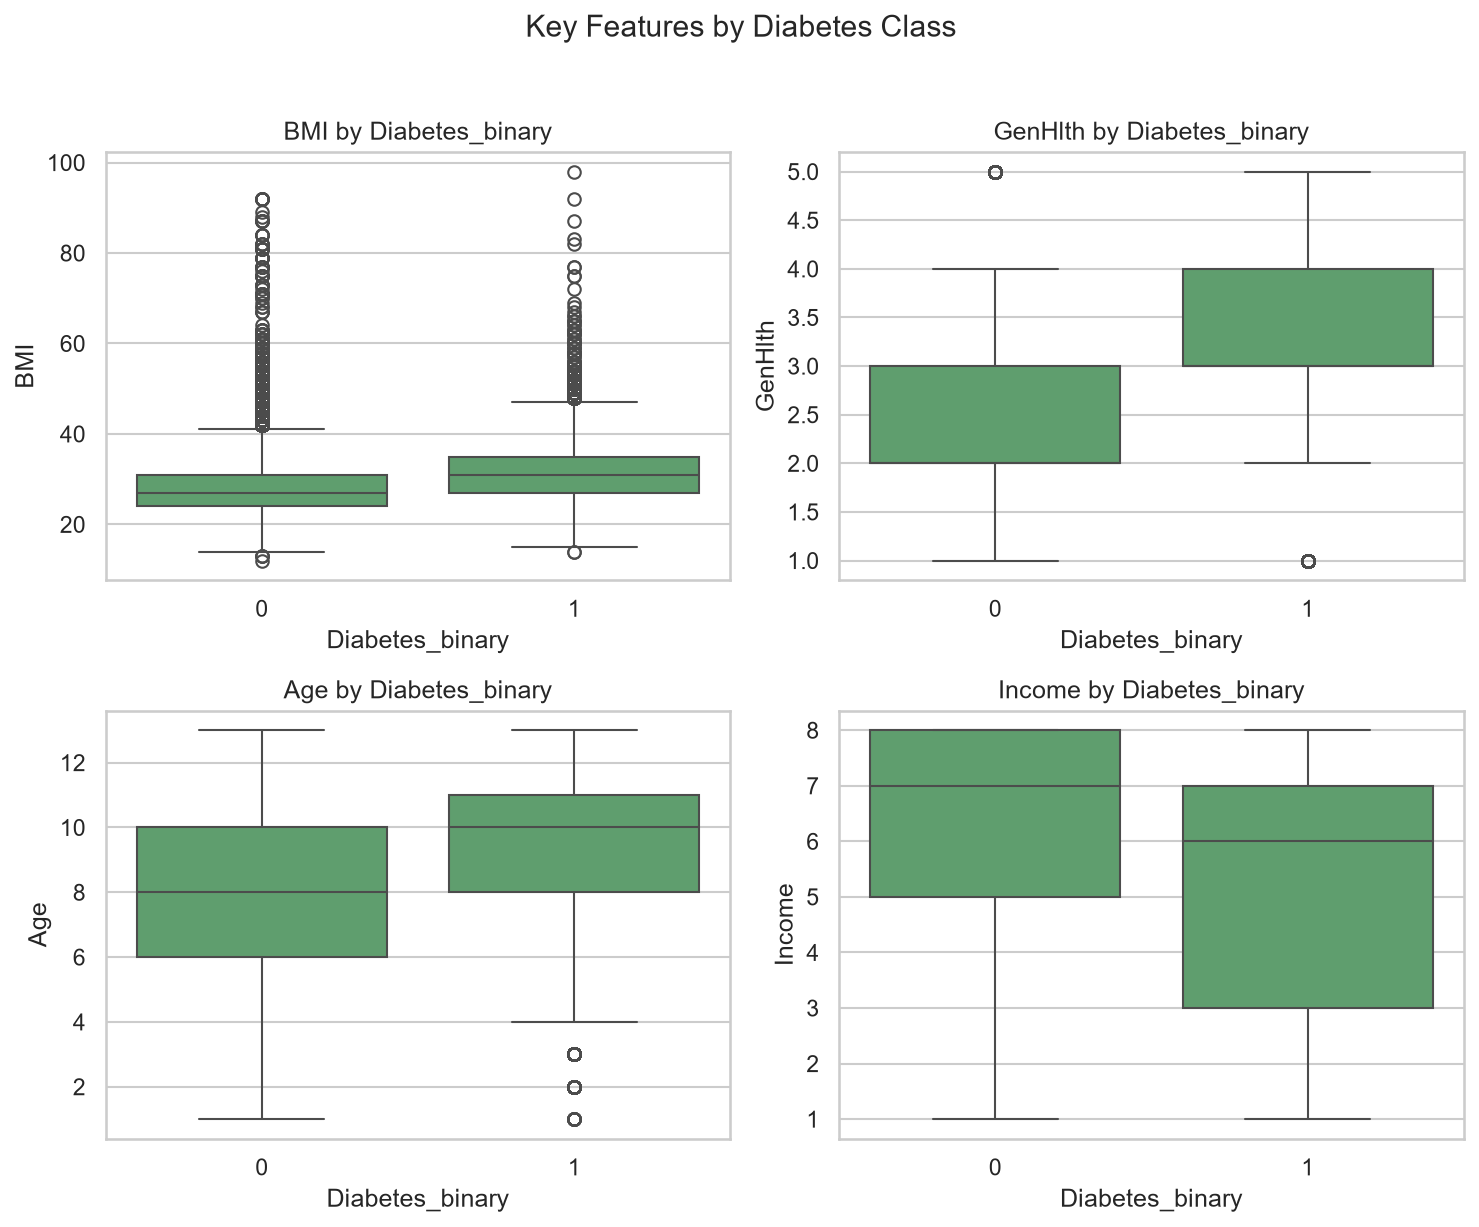
\includegraphics[width=0.85\textwidth]{feature_boxplots_by_class.png}
\caption{Boxplots of key features by class.}
\label{fig:box}
\end{figure}

\subsection{Benchmark metrics}\label{sec:analysis-bench}

Table~\ref{tab:bench} reports default class weights. Accuracy is high (0.82--0.84) for all models. Linear SVM achieves the best Accuracy (0.8416) and AUC (0.8070) but very low Recall (0.0973) and F1 (0.1675). KNN leads F1 (0.2964) with AUC 0.7087. Random forest and logistic regression rank between these extremes on F1 while staying near $0.80+$ AUC.

\begin{table}[htbp]
\centering
\caption{Model benchmark metrics (default class weights).}
\label{tab:bench}
\scriptsize
\begin{tabular}{lrrrrrr}
\toprule
Model & Accuracy & Precision & Recall & F1 & AUC & Train (s) \\
\midrule
KNN & 0.8170 & 0.4004 & 0.2352 & 0.2964 & 0.7087 & 0.060 \\
Decision Tree & 0.8352 & 0.4931 & 0.2034 & 0.2880 & 0.7706 & 0.041 \\
Random Forest & 0.8393 & 0.5284 & 0.1774 & 0.2656 & 0.8017 & 0.375 \\
Logistic Regression & 0.8410 & 0.5467 & 0.1710 & 0.2605 & 0.8067 & 0.018 \\
Linear SVM & 0.8416 & 0.6024 & 0.0973 & 0.1675 & 0.8070 & 0.026 \\
\bottomrule
\end{tabular}
\end{table}

\begin{figure}[htbp]
\centering
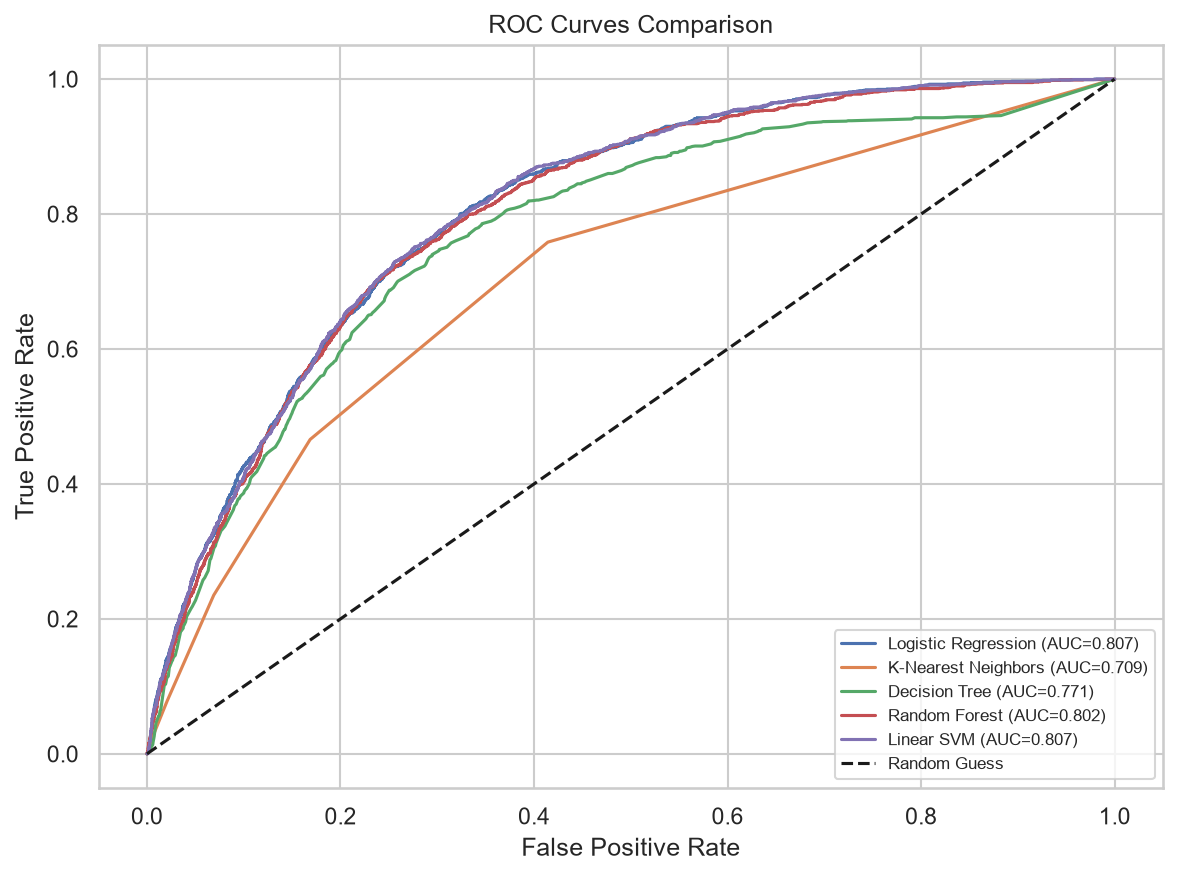
\includegraphics[width=0.85\textwidth]{roc_curves_benchmark.png}
\caption{ROC curves of five classical models.}
\label{fig:roc}
\end{figure}

\subsection{Best default-F1 model: KNN}\label{sec:analysis-knn}

KNN yields the highest default-threshold F1. Figure~\ref{fig:cm} shows substantial true positives but also many false positives---consistent with moderate Precision (0.4004) and Recall (0.2352). High Accuracy therefore hides missed positives; class weights or threshold tuning are needed for screening recall.

\begin{figure}[htbp]
\centering
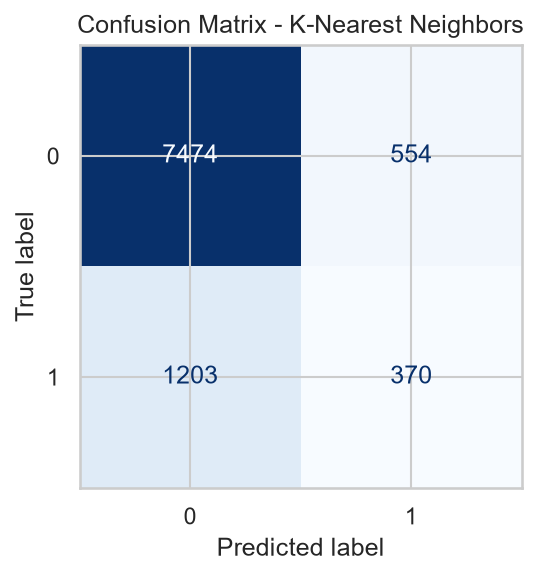
\includegraphics[width=0.72\textwidth]{confusion_matrix_best.png}
\caption{Confusion matrix of the best-F1 model (KNN).}
\label{fig:cm}
\end{figure}

\subsection{Random Forest feature importances}\label{sec:analysis-rf}

Figure~\ref{fig:rfimp} ranks Top-8 importances as BMI $>$ GenHlth $>$ Age $>$ HighBP $>$ Income $>$ HighChol $>$ DiffWalk $>$ HeartDiseaseorAttack. BMI rises to first place in the ensemble although GenHlth leads Pearson $|r|$, illustrating non-linear and interaction effects. Reporting both correlation and importance is more informative than either alone.

\begin{figure}[htbp]
\centering
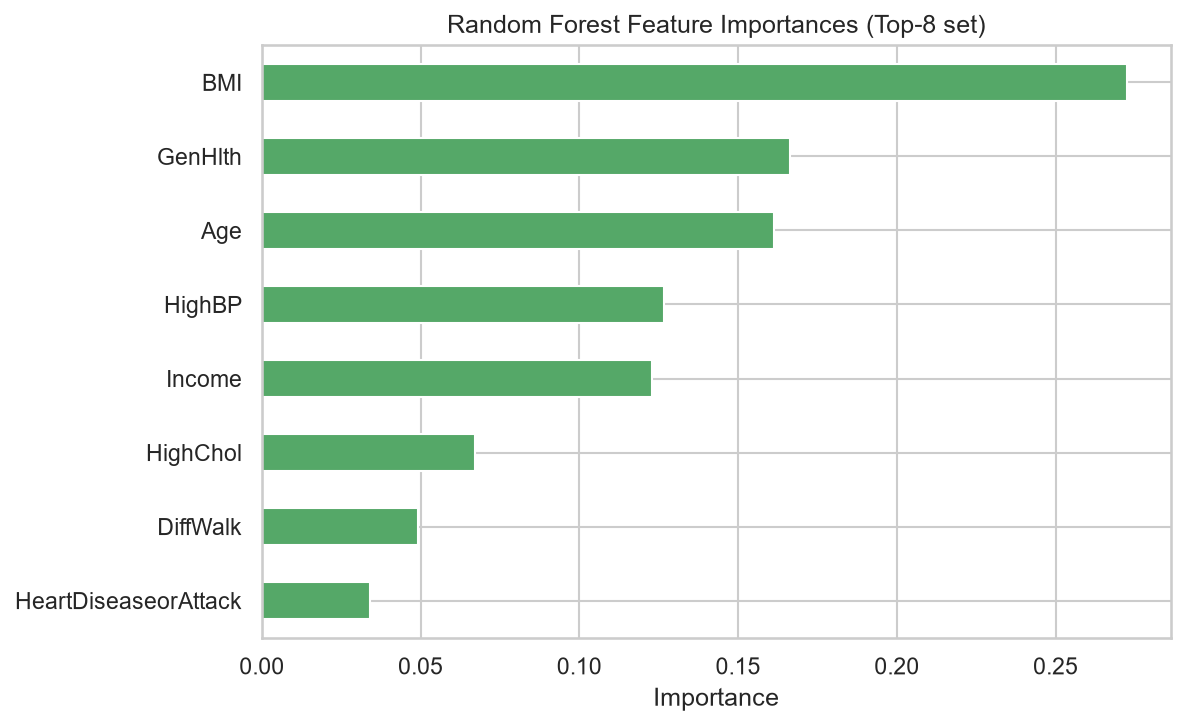
\includegraphics[width=0.85\textwidth]{rf_feature_importance.png}
\caption{Random Forest feature importances (Top-8).}
\label{fig:rfimp}
\end{figure}

\subsection{Class-weight ablation}\label{sec:analysis-ablation}

Table~\ref{tab:ablation} and Figure~\ref{fig:ablation} compare none vs.\ balanced weights for LR and RF. Balanced logistic regression increases Recall from 0.1710 to 0.7463 and F1 from 0.2605 to 0.4691 while Accuracy falls to 0.7233; AUC stays near 0.807. Balanced RF reaches Recall 0.6993 and F1 0.4673. Accuracy drops about ten percentage points---expected when minority detection improves.

\begin{table}[htbp]
\centering
\caption{Class-weight imbalance ablation (LR and RF).}
\label{tab:ablation}
\begin{tabular}{lrrrrr}
\toprule
Setting & Accuracy & Precision & Recall & F1 & AUC \\
\midrule
LR (none) & 0.8410 & 0.5467 & 0.1710 & 0.2605 & 0.8067 \\
LR (balanced) & 0.7233 & 0.3421 & 0.7463 & 0.4691 & 0.8074 \\
RF (none) & 0.8393 & 0.5284 & 0.1774 & 0.2656 & 0.8017 \\
RF (balanced) & 0.7388 & 0.3509 & 0.6993 & 0.4673 & 0.7976 \\
\bottomrule
\end{tabular}
\end{table}

\begin{figure}[htbp]
\centering
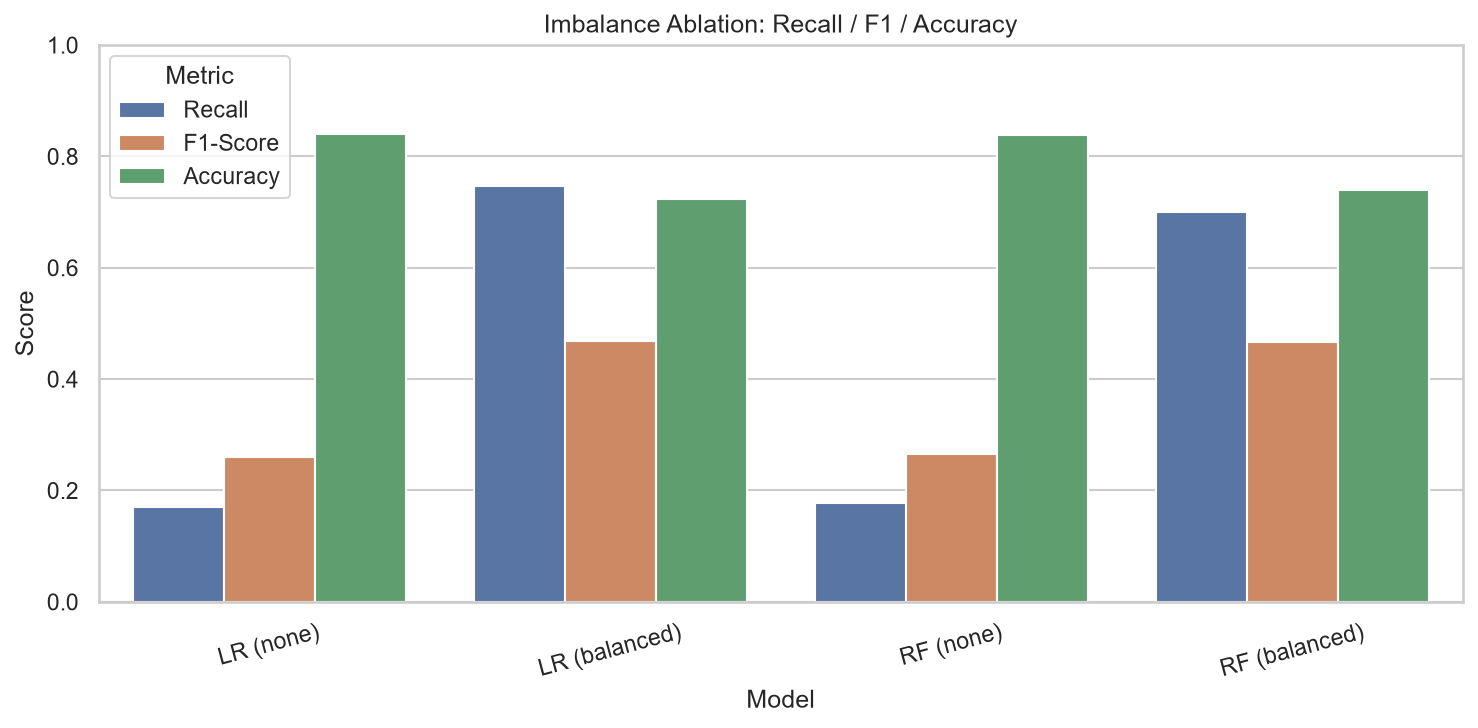
\includegraphics[width=0.85\textwidth]{imbalance_f1_recall_comparison.png}
\caption{Imbalance ablation: Recall / F1 / Accuracy.}
\label{fig:ablation}
\end{figure}

\subsection{Integrated discussion}\label{sec:analysis-discuss}

No single metric crowns one model for all goals. Under default weights, KNN wins F1 but misses many positives and trails in AUC; linear SVM and logistic regression rank risk well but suppress Recall. With balanced weights, logistic regression offers the best Recall/F1 compromise with stable AUC and fast training. For screening that penalizes false negatives, balanced logistic regression is the evidence-based recommendation---not the highest Accuracy model.

Limitations include Pearson Top-8 linear filtering, a single hold-out split, no SMOTE or threshold optimization, and \lstinline{LinearSVC} instead of kernel SVM.

%%%%%%%%%%%%%%%%%%%%%%%%%%%%%%%%%%%%%%%%%%%%%%%%%%%%%%%%%%%%%%%%%%%%%%
\section{Conclusions}\label{sec:conclusion}
%%%%%%%%%%%%%%%%%%%%%%%%%%%%%%%%%%%%%%%%%%%%%%%%%%%%%%%%%%%%%%%%%%%%%%

This benchmark on BRFSS-derived binary diabetes data shows that metric choice under imbalance changes which model is recommended. Key findings: (1)~83.6\%/16.4\% class balance inflates Accuracy while default Recall stays low; (2)~linear models lead AUC ($\sim$0.807) whereas KNN leads default F1 (0.2964) with weaker ranking; (3)~\lstinline{class_weight='balanced'} lifts LR Recall to 0.7463 and F1 to 0.4691 with modest AUC change; (4)~GenHlth, HighBP, BMI, and Age appear in both correlation and RF importance, with BMI prominent in the forest.

Methodologically, multi-metric reporting and explicit imbalance handling should be standard in comparative studies. Practically, screening workflows should state whether false negatives or false positives are costlier and compare weighted vs.\ unweighted models.

Future work may add nested cross-validation, probability calibration, SMOTE or undersampling, and interpretability tools (e.g., SHAP) on the full BRFSS feature set.

For the stated screening objective, balanced logistic regression is the best-supported choice in this protocol---better than optimizing default-threshold F1 alone or Accuracy alone.

%%%%%%%%%%%%%%%%%%%%%%%%%%%%%%%%%%%%%%%%%%%%%%%%%%%%%%%%%%%%%%%%%%%%%%
%% References (APA 6 author--year via natbib)
%%%%%%%%%%%%%%%%%%%%%%%%%%%%%%%%%%%%%%%%%%%%%%%%%%%%%%%%%%%%%%%%%%%%%%
\clearpage
\renewcommand{\refname}{References}
\begin{thebibliography}{99}

\bibitem[American Diabetes Association(2021)]{ADA2021}
American Diabetes Association. (2021).
Classification and diagnosis of diabetes: Standards of medical care in diabetes---2021.
\textit{Diabetes Care, 44}(Suppl.~1), S15--S33.
\url{https://doi.org/10.2337/dc21-S002}

\bibitem[Breiman(2001)]{Breiman2001}
Breiman, L. (2001).
Random forests.
\textit{Machine Learning, 45}(1), 5--32.
\url{https://doi.org/10.1023/A:1010933404324}

\bibitem[Centers for Disease Control and Prevention(2015)]{CDC2015}
Centers for Disease Control and Prevention. (2015).
\textit{Behavioral Risk Factor Surveillance System (BRFSS)}.
\url{https://www.cdc.gov/brfss/}

\bibitem[Chawla et~al.(2002)Chawla, Bowyer, Hall, and Kegelmeyer]{Chawla2002}
Chawla, N.~V., Bowyer, K.~W., Hall, L.~O., \& Kegelmeyer, W.~P. (2002).
SMOTE: Synthetic minority over-sampling technique.
\textit{Journal of Artificial Intelligence Research, 16}, 321--357.
\url{https://doi.org/10.1613/jair.953}

\bibitem[Cortes and Vapnik(1995)]{Cortes1995}
Cortes, C., \& Vapnik, V. (1995).
Support-vector networks.
\textit{Machine Learning, 20}(3), 273--297.
\url{https://doi.org/10.1007/BF00994018}

\bibitem[Fawcett(2006)]{Fawcett2006}
Fawcett, T. (2006).
An introduction to ROC analysis.
\textit{Pattern Recognition Letters, 27}(8), 861--874.
\url{https://doi.org/10.1016/j.patrec.2005.10.010}

\bibitem[He and Garcia(2009)]{He2009}
He, H., \& Garcia, E.~A. (2009).
Learning from imbalanced data.
\textit{IEEE Transactions on Knowledge and Data Engineering, 21}(9), 1263--1284.
\url{https://doi.org/10.1109/TKDE.2008.239}

\bibitem[Hosmer et~al.(2013)Hosmer, Lemeshow, and Sturdivant]{Hosmer2013}
Hosmer, D.~W., Lemeshow, S., \& Sturdivant, R.~X. (2013).
\textit{Applied logistic regression} (3rd~ed.).
Wiley.

\bibitem[James et~al.(2021)James, Witten, Hastie, and Tibshirani]{James2021}
James, G., Witten, D., Hastie, T., \& Tibshirani, R. (2021).
\textit{An introduction to statistical learning} (2nd~ed.).
Springer.
\url{https://doi.org/10.1007/978-1-0716-1418-1}

\bibitem[Teboul(n.d.)]{TeboulND}
Teboul, A. (n.d.).
\textit{Diabetes health indicators dataset}.
Kaggle.
\url{https://www.kaggle.com/datasets/alexteboul/diabetes-health-indicators-dataset}

\end{thebibliography}

%%%%%%%%%%%%%%%%%%%%%%%%%%%%%%%%%%%%%%%%%%%%%%%%%%%%%%%%%%%%%%%%%%%%%%
\begin{appendices}
%%%%%%%%%%%%%%%%%%%%%%%%%%%%%%%%%%%%%%%%%%%%%%%%%%%%%%%%%%%%%%%%%%%%%%

\section{List of Figures and Tables}\label{sec:app-lists}

\paragraph{List of Figures.}
\begin{itemize}[leftmargin=*]
  \item Figure~\ref{fig:classbalance}: Class balance of \texttt{Diabetes\_binary}
  \item Figure~\ref{fig:corr}: Pearson correlation heatmap
  \item Figure~\ref{fig:hist}: Selected feature histograms
  \item Figure~\ref{fig:box}: Boxplots of key features by class
  \item Figure~\ref{fig:roc}: ROC curves of five classical models
  \item Figure~\ref{fig:cm}: Confusion matrix of the best-F1 model (KNN)
  \item Figure~\ref{fig:rfimp}: Random Forest feature importances (Top-8)
  \item Figure~\ref{fig:ablation}: Imbalance ablation: Recall / F1 / Accuracy
\end{itemize}

\paragraph{List of Tables.}
\begin{itemize}[leftmargin=*]
  \item Table~\ref{tab:top8}: Pearson Top-8 features (training set)
  \item Table~\ref{tab:bench}: Model benchmark metrics
  \item Table~\ref{tab:ablation}: Class-weight imbalance ablation
\end{itemize}

\section{Reproduction notes}\label{sec:app-repro}

\begin{itemize}[leftmargin=*]
  \item Generate the 50k binary sample: \lstinline{python dataset/make_binary_50k.py}
  \item Run the experiment notebook: \lstinline{diabetes_ml_benchmark.ipynb}
  \item Fixed seeds and protocol: \lstinline{random_state=42}; \lstinline{test_size=0.2} (stratified); Pearson Top-8; \lstinline{StandardScaler} on training data only
  \item Install dependencies from \lstinline{requirements.txt} in the repository root
\end{itemize}

\noindent\textbf{Affidavit reminder.}
The signed Affidavit / Declaration of Academic Integrity must be attached at the end of the final LMS submission (Word/PDF). It is not generated in this manuscript source.

\end{appendices}

\end{document}
